\chapter{Literature Review}
With the development of science and technology, computer vision has gradually become popular in various engineering fields, leading the demand for exteroceptive sensors to increase in many different applications. In order to work with cameras, calibration is a critical stage and must be completed before capturing data \citep{Baker2003}. Therefore, various camera calibration methods have been published, suited to different project purposes. 

This chapter aims to provide a literature review of the previous camera calibration methods and discuss both the benefits and drawbacks of these methods. These related works are considered and analysed thoroughly to determine the most suitable approach for our project purpose.


\section{Camera calibration}
The actual camera calibration process is performed using calibration targets. These targets have a definite structure or sample, and their geometry is known for great precision. The camera will take the image of these calibration targets and then calculate the camera parameters (intrinsic and extrinsic) using math formulas and algorithms. One of the most notable publications on camera calibration is by \cite{Tsai1987}; he presented a two-stage camera calibration method using a mono view co-planar set of points. \cite{Zhang2000} proposed a calibration method using Closed-Form solution and Maximum-Likelihood Estimation. In this approach, his calibration target was a planar board with mostly square patterns and circle patterns at the corners, printed on paper and stuck onto the board. Research by \cite{Triggs1999} showed that the camera is required to capture at least five 3D points to one image to calibrate the extrinsic parameters. There is a drawback in Triggs' approach that these five 3D calibration dots had to belong to at least two different planes. 

\section{Multi-camera calibration}

\subsection{Stereo cameras}
Unlike calibrating a single camera, the calibration technique for a system with several cameras is more complicated and troublesome. In this situation, the intrinsic parameters must be calibrated independently, while the extrinsic calibration process should be implemented simultaneously. Various calibration methods have been published to estimate the extrinsic parameters of a multiple camera system. In research in 2003, Tomita and Ueshiba introduced a calibration method for two cameras using a planar calibration target. This pair of cameras would capture images of the target from two different orientations. Then, applying homography, both cameras would be intrinsically and extrinsically calibrated, and all the camera parameters would be solved \citep{Ueshiba2003}. With this method, although capturing images from two different orientations is enough, we can improve the accuracy of the calibration process by capturing more images from various locations. This method was then developed by calibrating a system with twelve cameras precisely.

\begin{figure}[ht]
\centering
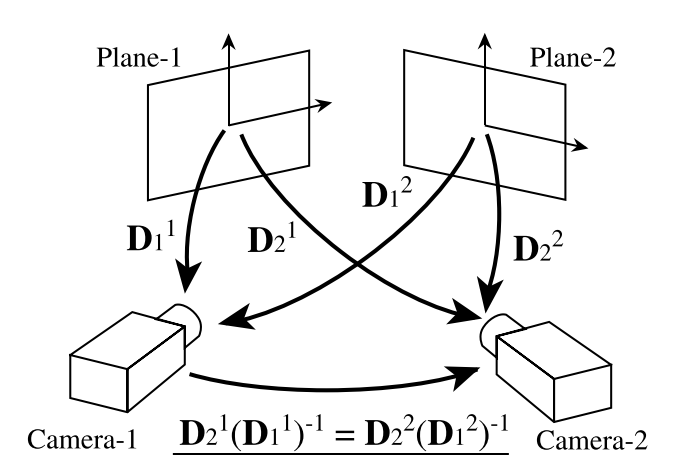
\includegraphics[width=0.7\textwidth]{Images/Tomita.png}
\caption{Ueshiba \& Tomita (2003) calibration method for overlapping camera system}
\end{figure}

\subsection{Non-overlapping Field of View cameras}
However, the calibration method of Tomita \& Ueshiba contained a significant drawback. This approach only works with a multiple overlapping camera system, which means all the cameras in the system have to be able to capture the 2D calibration target fully. In a research in 2016, \cite{Dong2016} introduced a method to calibrate a non-overlapping camera system. He used a wide planar board and printed encoded patterns with predefined positions (relative to the board origin). Therefore, each camera in the system does not need to capture the whole board during calibration, and camera can identify every single encoded pattern using a binary color-coding system. However, this method can only apply to extrinsically calibrate the camera system, so Dong had to get the intrinsic parameters of his cameras using Zhang's method.

\begin{figure}[ht]
\centering
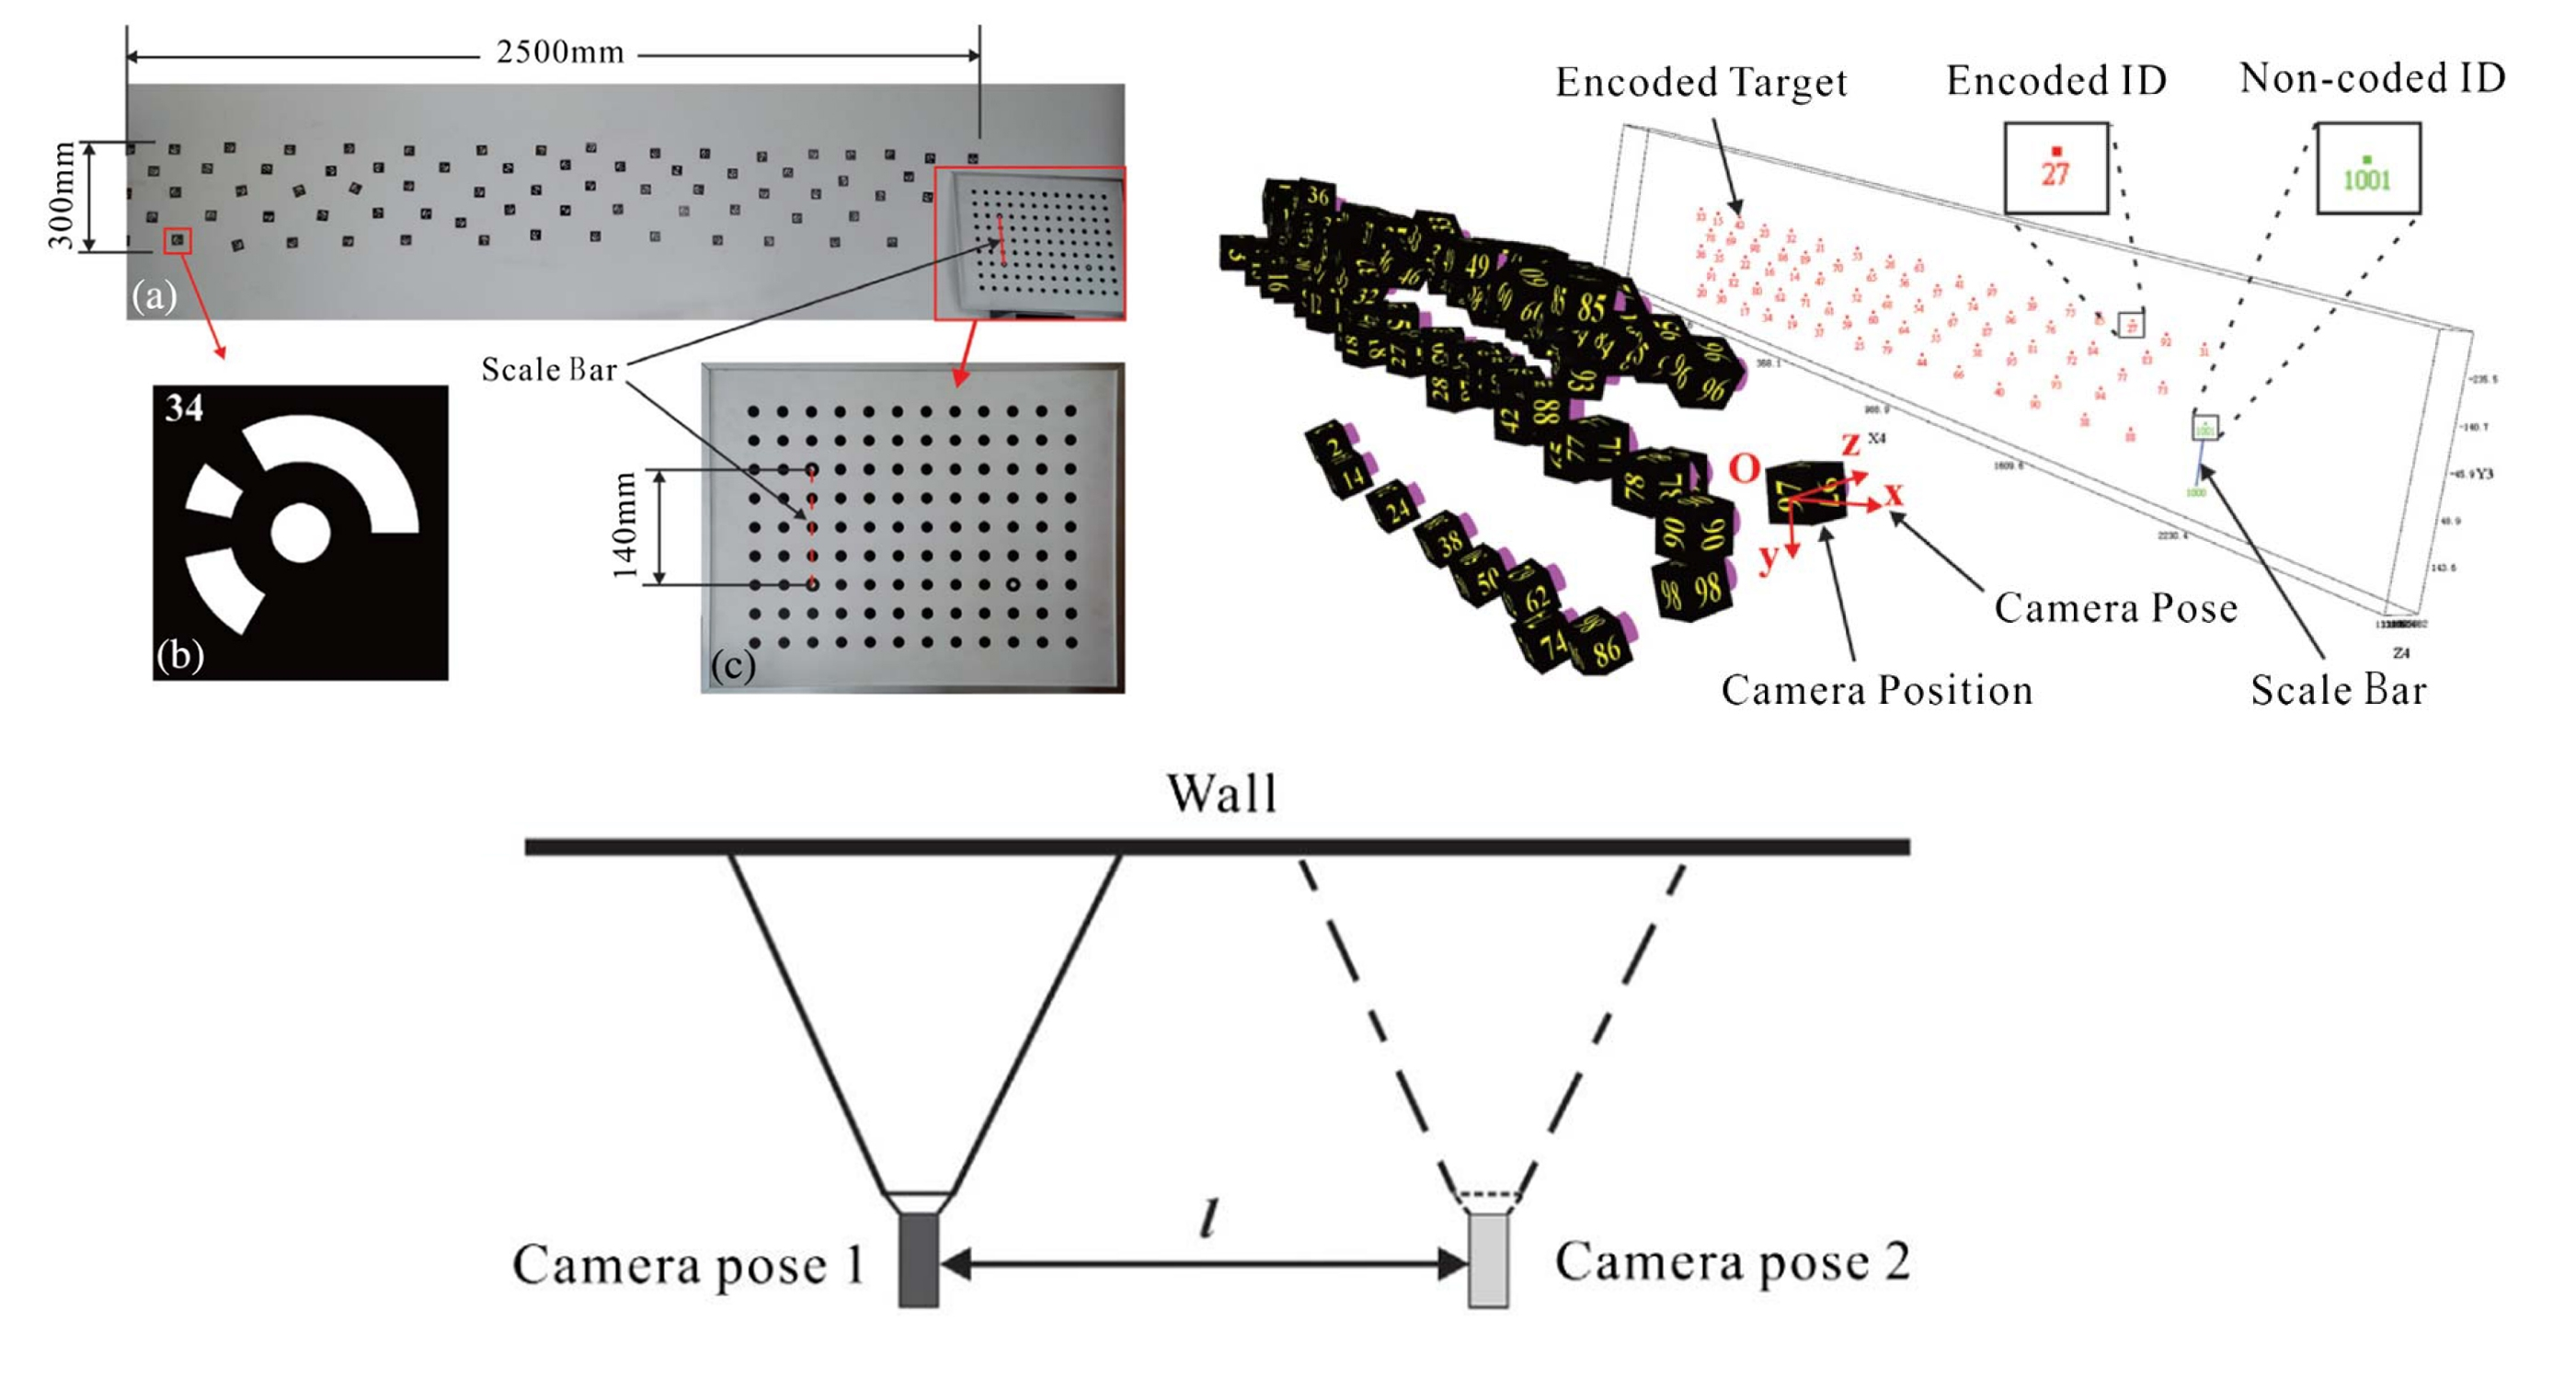
\includegraphics[width=0.8\textwidth]{Images/Dong (2016).jpg}
\caption{Dong et al. (2016) method for non-overlapping multiple camera system}
\end{figure}

Dong's calibration method still requires the cameras are placed close together with the same orientation due to the particular characteristics of the 2D calibration target. In fact, depending on the project purpose, there will be cases where the system contains cameras facing each other, and 2D calibration targets cannot be used because all cameras cannot thoroughly capture the planar calibration target. \cite{Marcon2017} introduced a calibration method that used a double-sided checkerboard. The cameras having opposite orientations independently capture one side of the board, and then the extrinsic parameters are estimated together with the displacement error between two sides of the board.

\begin{figure}[ht]
\centering
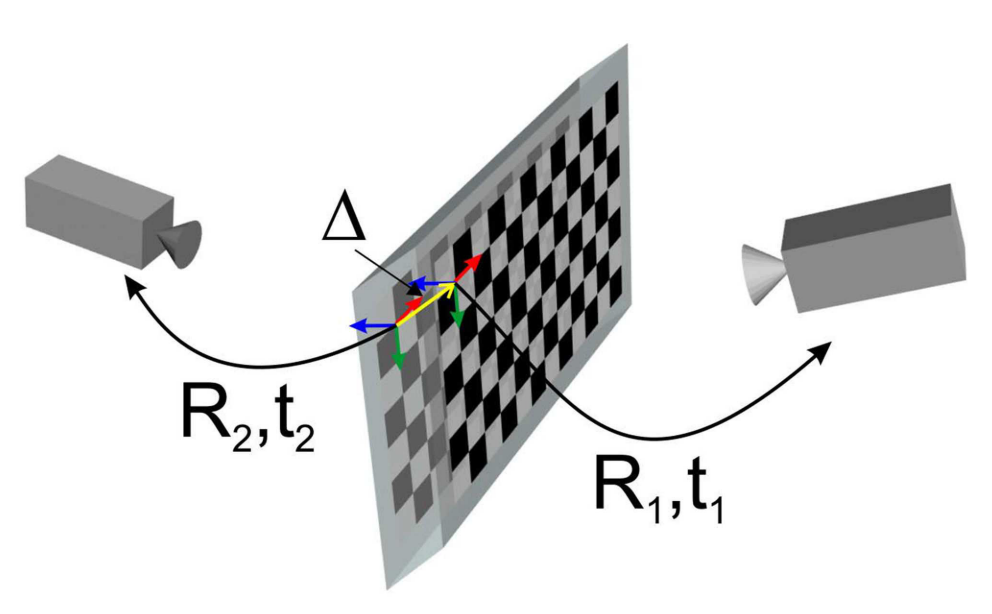
\includegraphics[width=1\textwidth]{Images/Marcon (2017).png}
\caption{Double-sided checkerboard of Marcon et al. (2017)}
\end{figure}

However, Marcon's (2017) approach could not solve the problem of cameras facing back to each other, for example, the airborne remote sensing camera system. Therefore, \cite{Yin2018} proposed a calibration method as a solution for these multi-camera systems. In his approach, he chose one camera as the origin reference frame, and then the extrinsic parameters would be the relative pose between each camera in the system to the reference camera. His method consisted of two stages: estimating the relative poses between every pair of cameras in this system and then calculating the extrinsic parameters based on optimising the re-projection errors using the Global Optimal Method. The results obtained were very positive: 0.001 radians and 0.08 millimetres on rotation and translation, respectively.

\begin{figure}[ht]
\centering
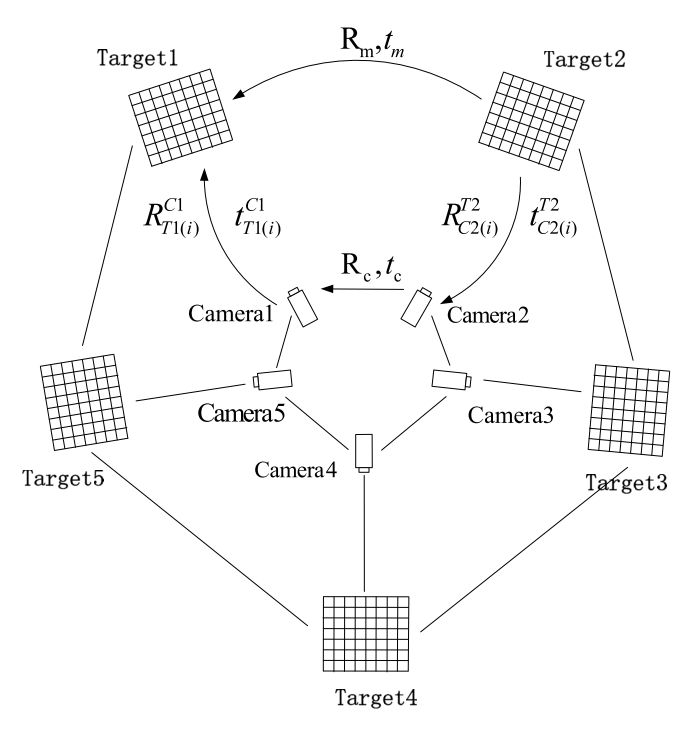
\includegraphics[width=0.9\textwidth]{Images/Yin et al. (2018).png}
\caption{Yin et al. (2018) calibration method}
\end{figure}

\clearpage
Additionally, several calibration methods use non-planar calibration targets or 3D calibration objects. \cite{Shen2011} published a technique using a sphere to calibrate a multi-camera system. They used eight 3D calibration dots, which are spherical with different colors, for the calibration of a system with twelve cameras. In this approach, each camera does not need to capture all eight dots in the calibration process, because just six calibration points are required to be captured by each camera once.



\begin{figure}[ht]
\centering
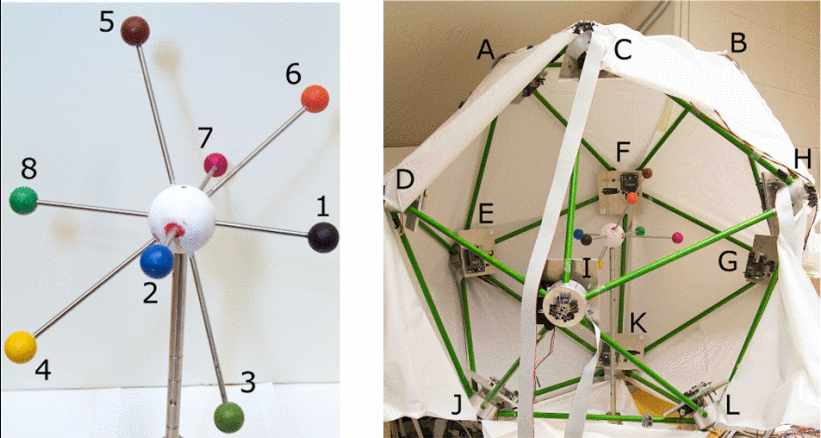
\includegraphics[width=1\textwidth]{Images/Shen (2011).png}
\caption{Spherical calibration targets of Shen \& Hornsey (2011)}
\end{figure}

\clearpage
\section{Fiducial markers}
Fiducial markers play an essential role in camera calibration. Fiducial marker defines visual sample targets within a physical environment that is discoverable and localisable by kinds of an exteroceptive sensor (camera, lidar...) \citep{Korthals2019}. Numerous types of fiducial markers were proposed in computer vision systems, such as ArUco markers \citep{Garrido-Jurado2014}, AprilTag \citep{Olson2011}, ARToolKit... Fiducial markers have been widely used in various vision applications, including camera calibration, robotics and augmented reality. Moreover, many support libraries have been provided to simplify the adoption of these markers.

\begin{figure}[ht]
\centering
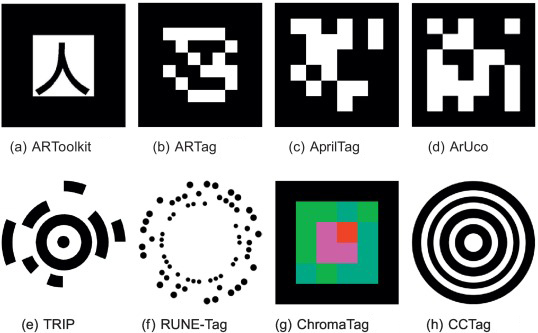
\includegraphics[width=1\textwidth]{Images/Fiducial markers.jpg}
\caption{Fiducial markers}
\end{figure}

\clearpage
\section{General Graph Optimisation}
To increase the accuracy of camera parameters during the calibration process, especially calibrating a multi-camera system, we should repeat the calibration procedure many times to optimise the result. The problem of graph optimisation has been researched extensively in several computer vision and robotics fields. \cite{Reinke2019} have proposed an extrinsic calibration method for a multi-camera system on legged robots based on factor graph optimisation. In their experiments, they captured a total of 1312 images, and after calibrating, their results had errors of about 2.03\% and 3.8\% on translation and rotation, respectively.

\begin{figure}[ht]
\centering
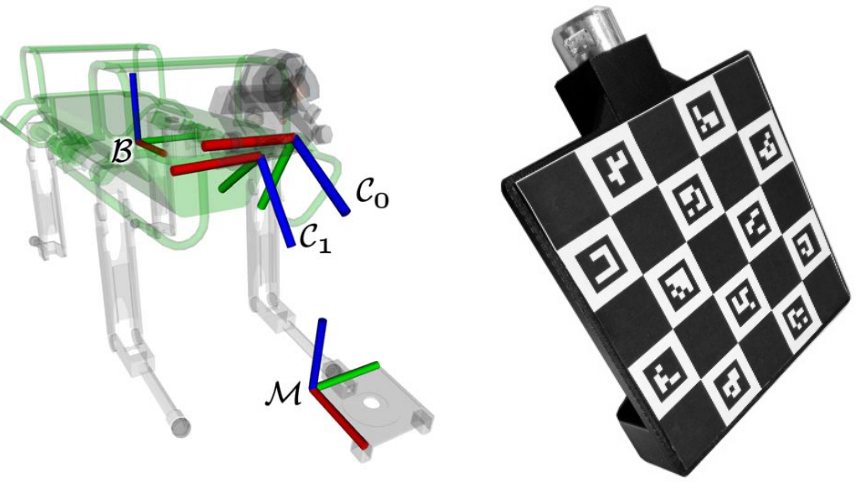
\includegraphics[width=0.8\textwidth]{Images/Reinke et al. (2019).png}
\caption{Multiple camera system on a legged robot}
\end{figure}